\subsection{Comparison of the isotropy groups of the cohomotoper and the coequalizer}

Let H be a quiver, let G be a groupoid, let \(\varphi\) and \(\psi\) be morphisms of quivers from H to G. Denote by \(\alpha\colon\mathrm{G}\to\mathrm{Coh}(\varphi,\psi)\) , \(\beta\colon\mathrm{Coh}(\varphi,\psi)\to\mathrm{Coeg}(\varphi,\psi)\) and \(\gamma\colon\mathrm{G}\to\mathrm{Coeg}(\varphi,\psi)\) the canonical morphisms of groupoids, and \(h\) the canonical homotopy relating \(\alpha\circ\varphi\) to \(\alpha\circ\psi\) . We summarize these notations by the following diagram

\pandocbounded{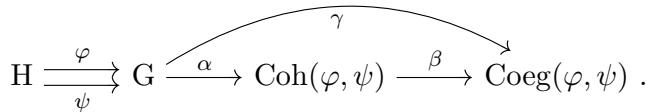
\includegraphics[keepaspectratio]{images/part002_030b7800.jpg}}

Throughout the rest of this section, \(n^{o}\), we assume that the frame of the pair \((\varphi,\psi)\) is a connected quiver and fix a vertex \(a_{0}\) of G. Consequently, the groupoids \(\mathrm{Coh}(\varphi,\psi)\) and \(\mathrm{Coeg}(\varphi,\psi)\) are transitive.

Denote by \(\Gamma\) the quiver \((\mathrm{Som}(\mathrm{G}), \mathrm{Som}(\mathrm{H}), \mathrm{Som}(\varphi), \mathrm{Som}(\psi))\) , \(\widetilde{\Gamma}\) the graph associated with \(\Gamma\), and let \(\Omega(\widetilde{\Gamma})\) be the set of finite sequences \((z_1, \ldots, z_n)\) of arrows of \(\widetilde{\Gamma}\) , with \(n \geqslant 1\) , such that the term of \(z_i\) is the origin of \(z_{i+1}\) if \(1 \leqslant i < n\) and that the term of \(z_n\) is the origin of \(z_1\) . In No. 1 we constructed a map \(\mathbf{z} \mapsto c(\mathbf{z})\) from the set \(\Omega(\widetilde{\Gamma})\) into the set of conjugacy classes of the group \(\mathrm{Coh}(\varphi, \psi)_{a_0}\) .

Denote by \(H \times_{G} H\) the equalizer in \(H \times H\) of the quiver morphisms \(\psi \circ pr_{1}\) and \(\varphi \circ pr_{2}\) . The set of its vertices is the set of pairs \((a, b)\) of vertices of H such that \(\psi(a) = \varphi(b)\) ; the set of its arrows is the set of pairs \((f, g)\) of arrows of H such that \(\psi(f) = \varphi(g)\) ; the origin of an arrow \((f, g)\) is the vertex \((o(f), o(g))\) and its endpoint is the vertex \((t(f), t(g))\) (cf. II, p. 153).

Finally, denote by \(\mathrm{Ker}(\varphi, \psi)\) the equalizer of \(\varphi\) and \(\psi\) ; recall (II, p. 165, example 2) that this is the subquiver of H whose vertices \(a\) are those such that \(\varphi(a) = \psi(a)\) and whose arrows are the \(f \in \mathrm{Fl}(\mathrm{H})\) such that \(\varphi(f) = \psi(f)\) .

PROPOSITION 4. --- Let \(\mu\colon\mathrm{H}\times_{\mathrm{G}}\mathrm{H}\to\mathrm{H}\) be a quiver morphism such that \(\varphi\circ\mu=\varphi\circ\mathrm{pr}_{1}\) and \(\psi\circ\mu=\psi\circ\mathrm{pr}_{2}\) . Suppose that, for every pair \((a,b)\) of vertices of H such that \(\varphi(a)=\varphi(b)\) , there exists a vertex \(c\) of H such that \(\varphi(c)=\psi(b)\) and \(a=\mu(b,c)\) .

  Let \(A_{1}\) be a set of vertices of \(\mathrm{Ker}(\varphi,\psi)\) meeting each of its connected components, and let \(Z_{1}\) be the set of elements of \(\Omega(\widetilde{\Gamma})\) of the form \(((a,1))\) , where \(a\in A_{1}\). Let \(A_{2}\) be a set of vertices of \(H\times_{G}H\) meeting every connected component of \(H\times_{G}H\) and let \(Z_{2}\) be the set of triples of the form \(((a,1),(b,1),(\mu(a,b),-1))\) , for \((a,b)\) ranging over \(A_{2}\) .

Then, \(\Omega(\widetilde{\Gamma})\) is the smallest distinguished subset of \(\Omega(\widetilde{\Gamma})\) which contains \(Z_1 \cup Z_2\). In particular, the conjugacy classes \(c(\mathbf{z})\) in \(\mathrm{Coh}(\varphi, \psi)_{a_0}\) , where \(\mathbf{z}\) runs through \(Z_1 \cup Z_2\) , generate the kernel of the canonical homomorphism \(\beta_{a_0}\) of \(\mathrm{Coh}(\varphi, \psi)_{a_0}\) to \(\mathrm{Coeg}(\varphi, \psi)_{\beta(a_0)}\) .

Denote by \(Z_{1}^{\prime}\) , \(Z_{2}^{\prime}\) and \(Z^{\prime}\) the smallest distinguished subsets of \(\Omega(\widetilde{\Gamma})\) respectively containing \(Z_{1}\) , \(Z_{2}\) and \(Z_{1} \cup Z_{2}\) (II, p. 197, def. 1). The aim is to prove that \(Z^{\prime}\) is equal to \(\Omega(\widetilde{\Gamma})\). By II, p. 199, corollary 1 of prop. 1 of II, p. 197, the last assertion of the proposition will follow from this.

Lemma 1. --- a) For every vertex \(a\) of \(\operatorname{Ker}(\varphi, \psi)\) , \(((a, 1))\) belongs to \(Z_1'\) .

\begin{enumerate}
\def\labelenumi{\alph{enumi})}
\setcounter{enumi}{1}
\item
  For every vertex \((a,b)\) of \(\mathrm{H}\times_{\mathrm{G}}\mathrm{H}\) , \(((a,1),(b,1),(\mu(a,b),-1))\) belongs to \(\mathbf{Z}_2^{\prime}\) .
\item
  Let \(A_{1}^{\prime}\) be the set of vertices \(a\) of \(\operatorname{Ker}(\varphi,\psi)\) such that \(((a,1))\) belongs to \(Z_{1}^{\prime}\) . We have \(A_{1}\subset A_{1}^{\prime}\) , by definition of \(Z_{1}^{\prime}\) . Let \(f\) be an arrow of \(\operatorname{Ker}(\varphi,\psi)\) , let \(a\) be its source and \(b\) its target. It follows from property (iv) in the definition of a distinguished subset (II, p. 197, def. 1) applied to the sequence \(((f,1))\) that \(a\in A_{1}^{\prime}\) is equivalent to \(b\in A_{1}^{\prime}\) . Since \(A_{1}\) meets every connected component of \(\operatorname{Ker}(\varphi,\psi)\) , we have \(A_{1}^{\prime}=\operatorname{Som}(\operatorname{Ker}(\varphi,\psi))\) , which is what had to be proved.
\item
  Let \(A_{2}^{\prime}\) be the set of vertices \((a,b)\) of \(H \times_{G} H\) such that the triple \(((a,1),(b,1),(\mu(a,b),-1))\) belongs to \(Z_{2}^{\prime}\) . By hypothesis, one has \(A_{2} \subset A_{2}^{\prime}\) . Since \(A_{2}\) meets each connected component of \(H \times_{G} H\) , it suffices to establish that, if there exists an arrow \((f,f^{\prime})\) joining a vertex \((a', b')\) to a vertex \((a, b)\) , then \((a, b)\) belongs to \(A_2'\) if and only if the same is true of \((a', b')\) .
\end{enumerate}

Let us set \(f'' = \mu(f, f')\) ; it is an arrow joining \(\mu(a', b')\) to \(\mu(a, b)\) and one has \(\varphi(f'') = \varphi(f)\) and \(\psi(f'') = \psi(f')\) . By condition (iv) in the definition of a distinguished subset of \(\Omega(\widetilde{\Gamma})\) (loc. cit.) applied to the sequence \(((f, 1), (f', 1), (f'', -1))\) , the two conditions

\begin{enumerate}
\def\labelenumi{(\roman{enumi})}
\item
  the triple \(((a,1),(b,1),(\mu (a,b), - 1))\) belongs to \(Z^{\prime}\) ;
\item
  the triple \(((a',1),(b',1),(\mu(a',b'),-1))\) belongs to \(Z'\) are equivalent. This shows that \((a,b)\) belongs to \(A_{2}'\) if and only if \((a',b')\) belongs to \(A_{2}'\) and concludes the proof of the lemma.
\end{enumerate}

We now prove by induction on the integer \(n \geqslant 1\) that every element \(((a_1, \varepsilon_1), (a_2, \varepsilon_2), \ldots, (a_n, \varepsilon_n))\) of \(\Omega(\widetilde{\Gamma})\) belongs to \(Z'\) .

\casehead{Case where \(n = 1\)}

Let \(((a,\varepsilon))\) be an element of \(\Omega(\tilde{\Gamma})\) of length 1. We have \(\varphi(a)=\psi(a)\) , whence \(((a,1))\in\mathbb{Z}'\). By Lemma 1, condition (ii) in the definition of a distinguished subset then implies that \(((a,-1))\) belongs to \(Z'\) .

\casehead{Case where \(n \geqslant 2\)}

By virtue of condition (ii) of a distinguished subset, it suffices to treat the case where \(\varepsilon_{2}=1\). Suppose that \(\varepsilon_{1}=1\) ; then, \((a_{1},a_{2})\) is a vertex of H \(\times_{G}H\) ; set \(a=\mu(a_{1},a_{2})\) ; by Lemma 1, the triple \(((a_{1},1),(a_{2},1),(a,-1))\) therefore belongs to \(Z'\). In the case where \(\varepsilon_{1}=-1\) , we have \(\varphi(a_{1})=\varphi(a_{2})\) ; one can therefore choose a vertex \(a\) of H such that \(\mu(a_{2},a)=a_{1}\) and the triple \(((a_{2},1),(a,1),(a_{1},-1))\) belongs to \(Z'\) , so the triple \(((a_{1},-1),(a_{2},1),(a,1))\) also belongs to \(Z'\), by virtue of condition (ii) in the definition of a distinguished subset.

Then, \(((a,\varepsilon_1),(a_3,\varepsilon_3),\ldots ,(a_n,\varepsilon_n))\) belongs to \(\Omega (\widetilde{\Gamma})\) and is of length \(n - 1\). By induction, this is an element of \(\mathbf{Z}'\) . Using conditions (i), (ii), and (iii) of the definition of a distinguished subset, we successively deduce that the elements

\[
\begin{array}{c} ((a _ {1}, \varepsilon_ {1}), (a _ {2}, 1), (a, - \varepsilon_ {1}), (a, \varepsilon_ {1}), (a _ {3}, \varepsilon_ {3}), \ldots , (a _ {n}, \varepsilon_ {n})), \\ ((a, - \varepsilon_ {1}), (a, \varepsilon_ {1}), (a _ {3}, \varepsilon_ {3}), \ldots , (a _ {n}, \varepsilon_ {n}), (a _ {1}, \varepsilon_ {1}), (a _ {2}, 1)), \\ ((a _ {3}, \varepsilon_ {3}), \ldots , (a _ {n}, \varepsilon_ {n}), (a _ {1}, \varepsilon_ {1}), (a _ {2}, 1)), \\ ((a _ {1}, \varepsilon_ {1}), (a _ {2}, 1), (a _ {3}, \varepsilon_ {3}), \ldots , (a _ {n}, \varepsilon_ {n})) \end{array}
\]

belong to Z'. This completes the proof of the proposition.

COROLLARY. --- a) With the notations of Proposition 4, suppose further that the map (Som(φ), Som(ψ)) from Som(H) into Som(G) × Som(G) is injective and that its image is the graph of an equivalence relation on Som(G). Then, for every vertex (a, b) of H \(\times_{G}\) H, there exists a unique vertex \(c_{a,b}\) of H such that \(\varphi(c_{a,b}) = \varphi(a)\) and \(\psi(c_{a,b}) = \psi(b)\) .

\begin{enumerate}
\def\labelenumi{\alph{enumi})}
\setcounter{enumi}{1}
\tightlist
\item
  Suppose further that for every arrow \((f, f')\) of H \(\times_{G}\) H, there exists an arrow \(f''\) of H such that \(\varphi(f'') = \varphi(f)\) and \(\psi(f'') = \psi(f')\) .
\end{enumerate}

Let A be a set of vertices of H \(\times_{G}\) H meeting each of its connected components. Then, the kernel of the morphism \(\beta_{a_{0}}\) is the smallest normal subgroup of \(\mathrm{Coh}(\varphi,\psi)_{a_{0}}\) which contains the conjugacy classes \(c((a,1),(b,1),(c_{a,b},-1))\) , for \((a,b)\in\mathrm{A}\) .

Let R be the equivalence relation on \(\operatorname{Som}(\mathrm{G})\) whose graph is the image of the mapping \((\operatorname{Som}(\varphi),\operatorname{Som}(\psi))\) . Let \((a,b)\) be a vertex of \(H\times_{G}H\) . One thus has \(\operatorname{R}\{\varphi(a),\psi(a)\}\) and \(\operatorname{R}\{\varphi(b),\psi(b)\}\) , whence \(\operatorname{R}\{\varphi(a),\psi(b)\}\) since \(\psi(a)=\varphi(b)\) . Hence, there exists a unique vertex \(c\) of H such that \(\varphi(c)=\varphi(a)\) and \(\psi(c)=\psi(b)\) ; it is denoted \(\mu(a,b)\) .

For every arrow \((f, f')\) of \(H\times_{G}H\), choose an arrow \(f''\) of H such that \(\varphi(f'') = \varphi(f)\) and \(\psi(f'') = \psi(f')\) and denote it \(\mu(f, f')\) .

We have thus defined a quiver morphism \(\mu\colon\mathrm{H}\times_{\mathrm{G}}\mathrm{H}\to\mathrm{H}\) such that \(\varphi\circ\mu=\varphi\circ\mathrm{pr}_{1}\) and \(\psi\circ\mu=\psi\circ\mathrm{pr}_{2}\) .

Let \((a,b)\) be a pair of vertices of H such that \(\varphi(a)=\varphi(b)\) . We have \(\mathrm{R}\{\varphi(a),\psi(a)\}\) and \(\mathrm{R}\{\varphi(b),\psi(b)\}\) , therefore \(\mathrm{R}\{\psi(b),\psi(a)\}\) . There consequently exists a unique vertex \(c\) of H such that \(\varphi(c)=\psi(b)\) and \(\psi(c)=\psi(a)\) . The vertex \(\mu(b,c)\) satisfies \(\varphi(\mu(b,c))=\varphi(b)=\varphi(a)\) and \(\psi(\mu(b,c))=\psi(c)=\psi(a)\) . We therefore have \(\mu(b,c)=a\) since the map \((\operatorname{Som}(\varphi),\operatorname{Som}(\psi))\) of \(\operatorname{Som}(\operatorname{H})\) into \(\operatorname{Som}(\operatorname{G})\times\operatorname{Som}(\operatorname{G})\) is injective.

Let \(A_{1}\) be the set of vertices of \(\operatorname{Ker}(\varphi,\psi)\) and let \(Z_{1}\) be the set of elements of \(\Omega(\widetilde{\Gamma})\) of the form \(((a,1))\) , for \(a\in A_{1}\) . Set \(A_{2}=A\) and let \(Z_{2}\) be the set of elements \(((a,1),(b,1),(\mu(a,b),-1))\) of \(\Omega(\widetilde{\Gamma})\) , for \((a,b)\in A_{2}\) . Denote by \(\widetilde{Z}\) (resp. \(\widetilde{Z}_{1}\), respectively \(\widetilde{Z}_{2}\)) the smallest distinguished subset of \(\Omega(\widetilde{\Gamma})\) containing \(Z_{1}\cup Z_{2}\) (resp. \(Z_{1}\), respectively \(Z_{2}\)).

Let \(a \in \mathrm{A}_1\). We have \(\varphi(a) = \psi(a)\) ; set \(x = \varphi(a)\). The vertex \(a\) is the unique vertex of H such that \(\varphi(a) = \psi(a) = x\). In particular, we have \(\mu(a, a) = a\). The triple \(((a, 1), (a, 1), (a, -1))\) therefore belongs to \(\mathbf{Z}_2\). It then follows from conditions (i) and (iii) in the definition of a distinguished subset that \(((a, 1))\) belongs to \(\widetilde{\mathbf{Z}}_2\). Consequently, we have \(\mathbf{Z}_1 \subset \widetilde{\mathbf{Z}}_2\) , whence \(\widetilde{\mathbf{Z}} = \widetilde{\mathbf{Z}}_2\) .

By Proposition 4, \(\Omega(\tilde{\Gamma})\) is the smallest distinguished subset of \(\Omega(\tilde{\Gamma})\) containing \(Z_{2}\), and the kernel of \(\beta_{a_{0}}\) is the smallest normal subgroup of \(\mathrm{Coh}(\varphi,\psi)_{a_{0}}\) which contains the conjugacy classes \(c(\mathbf{z})\) , for \(\mathbf{z}\in Z_{2}\) . Hence the corollary.

Example. --- Let X and R be topological spaces, let o and t be continuous maps from R to X, and let C be the set of pairs \((f,g)\in\mathrm{R}^{2}\) such that \(t(f)=o(g)\) in R and let m be a continuous map from C to R that makes the quiver \((\mathrm{X},\mathrm{R},o,t)\) a groupoid; suppose further that the map \(f\mapsto f^{-1}\) from R to R is continuous. The hypotheses of the proposition are then satisfied if one sets \(\mathrm{H}=\varpi(\mathrm{R})\) , \(\mathrm{G}=\varpi(\mathrm{X})\) , \(\varphi=\varpi(o)\) , \(\psi=\varpi(t)\) and \(\mu=\varpi(m)\) .

Suppose further that R is the graph of an equivalence relation on X, with the maps o and t being derived from the projections of \(X \times X\) in X by passing to subspaces. The hypotheses of the corollary are then satisfied.

Remark. --- *More generally, the hypotheses of the proposition are satisfied when (G, H, \(\varphi\) , \(\psi\) , \(\mu\) ) is a “groupoid of groupoids.” This means that G and H are groupoids, \(\varphi\) and \(\psi\) are morphisms of groupoids from H to G, making the quadruple (G, H, \(\varphi\) , \(\psi\) ) a “groupoid quiver”; finally, \(\mu\) is a composition law in this “quiver” given by a groupoid morphism H \(\times_{\mathrm{G}}\) H → H, satisfying a certain number of properties expressing the associativity of the law and the fact that every “arrow” is invertible. The reader will also note that the applications to the fundamental groupoid studied in this work all fall within this case.

